% ============================================================
% main.tex — Log-Based Recovery System (ADBMS Final Project)
% Compile with: pdflatex main.tex (run twice for TOC)
% ============================================================
\documentclass[12pt, a4paper]{report}

% ── Packages ─────────────────────────────────────────────────
\usepackage[utf8]{inputenc}
\usepackage[T1]{fontenc}
\usepackage[margin=1in]{geometry}
\usepackage{graphicx}
\usepackage{xcolor}
\usepackage{listings}
\usepackage{booktabs}
\usepackage{tabularx}
\usepackage{longtable}
\usepackage{amsmath}
\usepackage{hyperref}
\usepackage{fancyhdr}
\usepackage{titlesec}
\usepackage{setspace}
\usepackage{tocloft}
\usepackage{enumitem}
\usepackage{float}
\usepackage{caption}
\usepackage{subcaption}
\usepackage{mdframed}
\usepackage{tikz}
\usetikzlibrary{shapes.geometric, arrows.meta, positioning, fit}

% ── Hyperref setup ───────────────────────────────────────────
\hypersetup{
    colorlinks  = true,
    linkcolor   = blue!70!black,
    citecolor   = green!50!black,
    urlcolor    = blue!70!black,
    pdftitle    = {Log-Based Recovery System},
    pdfauthor   = {ADBMS Final Project},
}

% ── Page style ───────────────────────────────────────────────
\pagestyle{fancy}
\fancyhf{}
\fancyhead[L]{\small\textit{Log-Based Recovery System}}
\fancyhead[R]{\small\textit{ADBMS Final Project}}
\fancyfoot[C]{\thepage}
\renewcommand{\headrulewidth}{0.4pt}

% ── Chapter title formatting ─────────────────────────────────
\titleformat{\chapter}[display]
  {\normalfont\huge\bfseries\color{blue!70!black}}
  {\chaptertitlename\ \thechapter}{10pt}{\Huge}
\titlespacing*{\chapter}{0pt}{-10pt}{20pt}

% ── Line spacing ─────────────────────────────────────────────
\onehalfspacing

% ── Code listing style ───────────────────────────────────────
\definecolor{codebg}{rgb}{0.96,0.96,0.96}
\definecolor{codeframe}{rgb}{0.7,0.7,0.9}
\definecolor{keyword}{rgb}{0.0,0.3,0.7}
\definecolor{comment}{rgb}{0.3,0.5,0.3}
\definecolor{string}{rgb}{0.6,0.1,0.1}

\lstdefinestyle{sqlstyle}{
    language     = SQL,
    backgroundcolor = \color{codebg},
    frame        = single,
    rulecolor    = \color{codeframe},
    basicstyle   = \ttfamily\small,
    keywordstyle = \color{keyword}\bfseries,
    commentstyle = \color{comment}\itshape,
    stringstyle  = \color{string},
    breaklines   = true,
    numbers      = left,
    numberstyle  = \tiny\color{gray},
    captionpos   = b,
    tabsize      = 4,
}

\lstdefinestyle{pythonstyle}{
    language     = Python,
    backgroundcolor = \color{codebg},
    frame        = single,
    rulecolor    = \color{codeframe},
    basicstyle   = \ttfamily\small,
    keywordstyle = \color{keyword}\bfseries,
    commentstyle = \color{comment}\itshape,
    stringstyle  = \color{string},
    breaklines   = true,
    numbers      = left,
    numberstyle  = \tiny\color{gray},
    captionpos   = b,
    tabsize      = 4,
}

\lstdefinestyle{jsonstyle}{
    language     = {},
    backgroundcolor = \color{codebg},
    frame        = single,
    rulecolor    = \color{codeframe},
    basicstyle   = \ttfamily\small,
    stringstyle  = \color{string},
    breaklines   = true,
    captionpos   = b,
}

% ── Custom box for notes ─────────────────────────────────────
\newmdenv[
  linecolor   = blue!40,
  backgroundcolor = blue!5,
  roundcorner = 5pt,
  innertopmargin    = 8pt,
  innerbottommargin = 8pt,
]{conceptbox}

% ── Front matter command ─────────────────────────────────────
\newcommand{\HRule}{\rule{\linewidth}{0.5mm}}

% ============================================================
\begin{document}

% ── Title Page ───────────────────────────────────────────────
\begin{titlepage}
\begin{center}

\textsc{\large University of Engineering and Technology}\\[0.3cm]
\textsc{\large Department of Computer Science}\\[0.5cm]
\textsc{Advanced Database Management Systems (CS-4XX)}\\[0.3cm]
\textsc{Final Project Report}\\[1.5cm]

\HRule\\[0.5cm]
{\huge \bfseries Log-Based Recovery System}\\[0.3cm]
{\large \bfseries Using PostgreSQL and MongoDB}\\[0.3cm]
\HRule\\[1.5cm]

\begin{minipage}{0.48\textwidth}
  \begin{flushleft}
    \textbf{Submitted by:}\\[0.2cm]
    Muhammad Abrar\\
    Roll No: 2024-CS-59\\[0.5cm]
    \textbf{Session:} 2024--2028\\
    \textbf{Semester:} 4th
  \end{flushleft}
\end{minipage}
\hfill
\begin{minipage}{0.48\textwidth}
  \begin{flushright}
    \textbf{Submitted to:}\\[0.2cm]
    [Instructor Name]\\
    Assistant Professor\\
    Dept. of Computer Science\\[0.5cm]
    \textbf{Date:} May 2026
  \end{flushright}
\end{minipage}

\vfill

\begin{figure}[H]
  \centering
  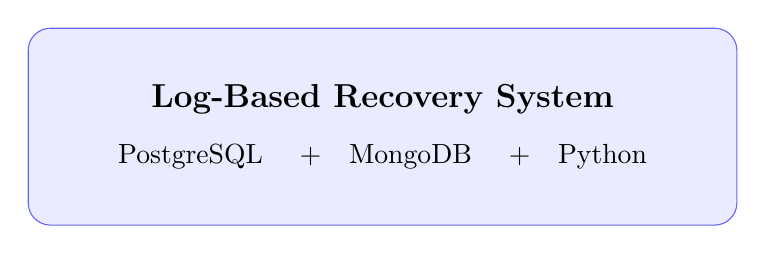
\begin{tikzpicture}
    \node[draw=blue!60, rounded corners=8pt, fill=blue!8,
          minimum width=9cm, minimum height=2.5cm, align=center,
          font=\bfseries\large] {
      Log-Based Recovery System\\[6pt]
      {\normalfont\normalsize PostgreSQL \quad+\quad MongoDB \quad+\quad Python}
    };
  \end{tikzpicture}
\end{figure}

\vfill
{\small Submitted in partial fulfillment of the requirements for the\\
Bachelor of Science in Computer Science degree.}

\end{center}
\end{titlepage}

% ── Certificate Page ─────────────────────────────────────────
\chapter*{Certificate}
\addcontentsline{toc}{chapter}{Certificate}
\thispagestyle{plain}

\vspace{1cm}
This is to certify that the project report titled:

\vspace{0.5cm}
\begin{center}
{\large \bfseries ``Log-Based Recovery System Using PostgreSQL and MongoDB''}
\end{center}
\vspace{0.5cm}

has been submitted by \textbf{Muhammad Abrar (Roll No: 2024-CS-59)} in partial
fulfillment of the requirements for the degree of Bachelor of Science in
Computer Science. The work is original and has been completed under my
supervision for the course \textbf{Advanced Database Management Systems (ADBMS)}.

\vspace{3cm}
\begin{minipage}{0.45\textwidth}
  \hrule\vspace{0.3cm}
  \textbf{Supervisor's Signature}\\[0.2cm]
  [Instructor Name]\\
  Department of Computer Science
\end{minipage}
\hfill
\begin{minipage}{0.45\textwidth}
  \hrule\vspace{0.3cm}
  \textbf{Student's Signature}\\[0.2cm]
  Muhammad Abrar\\
  Roll No: 2024-CS-59
\end{minipage}

% ── Declaration ──────────────────────────────────────────────
\chapter*{Declaration}
\addcontentsline{toc}{chapter}{Declaration}
\thispagestyle{plain}

I, \textbf{Muhammad Abrar}, Roll No \textbf{2024-CS-59}, hereby declare that
the project report titled \textit{``Log-Based Recovery System Using PostgreSQL
and MongoDB''} is my own work and has been written by me. All sources of
information used in this report are duly cited and acknowledged. This project
has not been submitted for any other degree or examination.

\vspace{2cm}
\begin{flushright}
  \hrule\vspace{0.3cm}
  Muhammad Abrar\\
  Roll No: 2024-CS-59\\
  Date: May 2026
\end{flushright}

% ── Acknowledgement ──────────────────────────────────────────
\chapter*{Acknowledgement}
\addcontentsline{toc}{chapter}{Acknowledgement}
\thispagestyle{plain}

I would like to express my sincere gratitude to my course instructor for
providing guidance and insights throughout this project. The concepts of
Write-Ahead Logging, crash recovery, and polyglot persistence introduced in
the \textbf{Advanced Database Management Systems} course formed the foundation
of this implementation.

I would also like to thank the open-source communities behind
\textbf{PostgreSQL} and \textbf{MongoDB} whose detailed documentation made
understanding transaction management and NoSQL logging much easier.

Finally, I thank my fellow students for their constructive feedback during the
project development phase.

% ── Abstract ─────────────────────────────────────────────────
\chapter*{Abstract}
\addcontentsline{toc}{chapter}{Abstract}
\thispagestyle{plain}

This project presents a simplified \textbf{Log-Based Recovery System} built
for educational demonstration of core Advanced Database Management Systems
(ADBMS) concepts. The system uses a \textbf{hybrid database architecture}
combining PostgreSQL for structured transactional banking data and MongoDB for
flexible Write-Ahead Log (WAL) storage.

The implementation simulates real-world database recovery scenarios including
transaction commits, rollbacks, system crashes, and recovery through
\textbf{Undo} and \textbf{Redo} operations. A Python-based recovery module
coordinates both databases, following a simplified ARIES-inspired three-phase
recovery process: Analysis, Undo, and Redo.

The project demonstrates key ADBMS concepts including ACID properties,
Write-Ahead Logging, transaction lifecycle management, crash simulation,
and \textbf{polyglot persistence} --- the use of multiple database technologies
in a single system, each chosen for its strengths.

The banking domain is used as a practical scenario to make abstract recovery
concepts tangible and easy to demonstrate. The system is designed to be
undergraduate-level, practical to implement within one week, and suitable for
viva and presentation.

\vspace{0.5cm}
\noindent\textbf{Keywords:} Write-Ahead Logging, Undo/Redo Recovery, PostgreSQL,
MongoDB, ACID Properties, Polyglot Persistence, Crash Recovery, ADBMS.

% ── Table of Contents ────────────────────────────────────────
\tableofcontents
\listoffigures
\listoftables

% ── Include Chapters ─────────────────────────────────────────
% ============================================================
% ch01_introduction.tex
% Chapters: Introduction, Problem Statement, Objectives,
%           Literature Review, Existing vs Proposed System
% ============================================================

\chapter{Introduction}

\section{Background}

Modern database management systems must handle unexpected failures gracefully.
When a system crashes mid-transaction, data can be left in an inconsistent
state --- some changes applied, others lost. The mechanism that prevents
permanent data loss is called \textbf{database recovery}, and it relies on
\textbf{transaction logs} to determine what was committed and what was not.

This project implements a simplified \textbf{Log-Based Recovery System} that
demonstrates these concepts using two databases working together:

\begin{itemize}
  \item \textbf{PostgreSQL} --- a relational database storing structured
        banking data (accounts, customers, transactions).
  \item \textbf{MongoDB} --- a document database storing Write-Ahead Log
        (WAL) entries that record every transaction before it is applied.
\end{itemize}

The combination of two database technologies in one system is called
\textbf{polyglot persistence} --- a core concept in modern ADBMS.

\section{Motivation}

Traditional textbook explanations of database recovery are often abstract.
This project makes recovery concepts tangible by:

\begin{itemize}
  \item Simulating real crashes during active transactions
  \item Showing exactly what an UNCOMMITTED log looks like in MongoDB
  \item Demonstrating how \textit{old\_balance} and \textit{new\_balance}
        in a WAL log enable Undo and Redo operations
  \item Running a recovery process that restores database consistency
\end{itemize}

The banking domain (deposits, withdrawals, transfers) provides a familiar
scenario where inconsistency --- such as money being deducted without being
credited --- is easy to understand and verify.

\section{Scope of the Project}

\begin{conceptbox}
\textbf{This project is educational, not production-grade.}
The goal is to demonstrate ADBMS concepts clearly at undergraduate level,
not to implement a full DBMS recovery engine.
\end{conceptbox}

\noindent The scope includes:
\begin{itemize}
  \item Six PostgreSQL tables for banking data
  \item Three MongoDB collections for WAL and recovery logs
  \item Python modules for transactions, crash simulation, and recovery
  \item A simplified three-phase recovery process inspired by ARIES
\end{itemize}

The scope excludes: full ARIES internals, LSN chains, buffer pool management,
distributed recovery, and multi-user concurrency control.

% ────────────────────────────────────────────────────────────
\chapter{Problem Statement}

Traditional relational databases are vulnerable during system crashes.
When a database process is interrupted mid-transaction, two types of
problems arise:

\begin{enumerate}
  \item \textbf{Dirty writes} --- changes applied to disk that were never
        committed (should be undone).
  \item \textbf{Lost commits} --- changes that were committed logically but
        not yet flushed to disk before the crash (should be redone).
\end{enumerate}

Without a recovery mechanism, the database is left in an inconsistent state.
For a banking system, this could mean:

\begin{itemize}
  \item A withdrawal deducted from the sender's account but the receiver's
        credit was never applied.
  \item A deposit appearing committed in the application but lost from
        the database storage.
  \item Balance values that match neither the pre-transaction state nor
        the post-transaction state.
\end{itemize}

\noindent\textbf{The central problem this project solves:}

\begin{conceptbox}
How can a database system detect and repair inconsistencies caused by a
crash, using only the information available in transaction log records?
\end{conceptbox}

% ────────────────────────────────────────────────────────────
\chapter{Objectives}

The primary objectives of this project are:

\begin{enumerate}
  \item \textbf{Implement Write-Ahead Logging (WAL)} --- Every transaction
        writes a log record to MongoDB \textit{before} applying changes to
        PostgreSQL.

  \item \textbf{Simulate Crashes} --- Inject a system crash mid-transaction
        to create an inconsistent database state for recovery testing.

  \item \textbf{Implement UNDO Recovery} --- Identify UNCOMMITTED transactions
        from WAL logs and restore \textit{old\_balance} in PostgreSQL.

  \item \textbf{Implement REDO Recovery} --- Identify COMMITTED transactions
        whose PostgreSQL changes were lost and re-apply \textit{new\_balance}.

  \item \textbf{Demonstrate Polyglot Persistence} --- Use PostgreSQL and
        MongoDB together, each for what it does best.

  \item \textbf{Provide a Practical Demo} --- Create a menu-driven Python
        application that demonstrates all concepts interactively.
\end{enumerate}

\noindent\textbf{ADBMS concepts covered:}

\begin{table}[H]
\centering
\caption{ADBMS Concepts and Their Implementation}
\begin{tabularx}{\textwidth}{lX}
\toprule
\textbf{Concept} & \textbf{How Demonstrated} \\
\midrule
Transactions & Python TransactionManager with explicit COMMIT/ROLLBACK \\
ACID Properties & Atomicity via rollback; Durability via WAL \\
Write-Ahead Logging & MongoDB log written before every PostgreSQL update \\
Undo Recovery & old\_balance restored for UNCOMMITTED logs \\
Redo Recovery & new\_balance re-applied for lost COMMITTED changes \\
Crash Recovery & CrashSimulator raises exception before COMMIT \\
Polyglot Persistence & PostgreSQL for data + MongoDB for logs \\
\bottomrule
\end{tabularx}
\end{table}

% ────────────────────────────────────────────────────────────
\chapter{Literature Review}

\section{Database Transaction Management}

A \textbf{transaction} is a logical unit of work that must be executed
completely or not at all. The ACID properties --- Atomicity, Consistency,
Isolation, and Durability --- define the guarantees that a reliable
transaction system must provide \cite{ramakrishnan2002}.

\begin{itemize}
  \item \textbf{Atomicity}: A transaction either completes fully or has
        no effect. PostgreSQL achieves this through \texttt{COMMIT} and
        \texttt{ROLLBACK}.
  \item \textbf{Consistency}: The database moves from one valid state to
        another. CHECK constraints and foreign keys enforce this.
  \item \textbf{Isolation}: Concurrent transactions do not interfere.
        PostgreSQL uses MVCC (Multi-Version Concurrency Control).
  \item \textbf{Durability}: Committed changes survive crashes. WAL logging
        ensures durability by writing changes to a log before applying them.
\end{itemize}

\section{Write-Ahead Logging}

Write-Ahead Logging (WAL) is the fundamental technique for ensuring database
durability \cite{mohan1992}. The WAL rule states:

\begin{conceptbox}
\textbf{WAL Rule}: A log record describing a data change must be written to
stable storage \textit{before} the data change itself is written.
\end{conceptbox}

In our system, ``stable storage'' is MongoDB and ``data change'' is the
PostgreSQL balance update. Every transaction follows this sequence:
\begin{enumerate}
  \item Write log to MongoDB (UNCOMMITTED)
  \item Update PostgreSQL
  \item COMMIT PostgreSQL
  \item Update MongoDB log to COMMITTED
\end{enumerate}

\section{ARIES Recovery Algorithm}

The ARIES (Algorithm for Recovery and Isolation Exploiting Semantics) algorithm
\cite{mohan1992} is the industry standard for crash recovery in relational
databases. It operates in three phases:

\begin{enumerate}
  \item \textbf{Analysis Phase}: Scan the log to identify committed and
        uncommitted transactions at crash time.
  \item \textbf{Redo Phase}: Re-apply all logged changes to ensure the
        database reflects all committed operations.
  \item \textbf{Undo Phase}: Reverse all changes made by uncommitted
        transactions.
\end{enumerate}

Our project implements a simplified version of this three-phase approach
without LSN chains, dirty page tables, or checkpoint records.

\section{Polyglot Persistence}

Polyglot persistence refers to using multiple database technologies within
a single application, each chosen for its strengths \cite{fowler2012}.
NoSQL databases like MongoDB are well-suited for flexible, high-speed log
storage because:

\begin{itemize}
  \item Schema-free documents can store variable metadata per log entry
  \item Insert operations are fast and do not require transaction overhead
  \item Rich query capabilities allow efficient log filtering by status
  \item MongoDB is independent of the PostgreSQL transaction — a failed
        PG transaction does not affect the MongoDB log
\end{itemize}

% ────────────────────────────────────────────────────────────
\chapter{Existing System vs Proposed System}

\section{Existing Approaches}

Traditional database recovery approaches have significant limitations for
educational purposes:

\begin{table}[H]
\centering
\caption{Existing vs Proposed System Comparison}
\begin{tabularx}{\textwidth}{lXX}
\toprule
\textbf{Aspect} & \textbf{Existing/Traditional} & \textbf{Proposed System} \\
\midrule
Log Storage & Binary log files on disk & MongoDB JSON documents \\
Log Format & Internal binary format & Human-readable JSON \\
Recovery & Automated, invisible to user & Explicit, demonstrable steps \\
Complexity & Full ARIES with LSNs & Simplified 3-phase approach \\
Observability & Cannot inspect logs easily & Query logs with mongosh \\
Database Type & Single RDBMS & Hybrid PostgreSQL + MongoDB \\
Educational Use & Not designed for teaching & Specifically for ADBMS demos \\
Crash Testing & Requires actual system crash & Python Exception injection \\
\bottomrule
\end{tabularx}
\end{table}

\section{Advantages of the Proposed System}

\begin{enumerate}
  \item \textbf{Transparency}: Every log entry is a readable JSON document
        that students can inspect and understand.
  \item \textbf{Demonstrability}: The crash and recovery sequence is
        observable step-by-step in the terminal.
  \item \textbf{Concept Clarity}: The separation of WAL (MongoDB) and data
        (PostgreSQL) makes the WAL principle visually clear.
  \item \textbf{Practical Implementation}: Runs on a single laptop with
        freely available software.
\end{enumerate}

% ============================================================
% ch02_architecture.tex
% System Architecture and ER Diagram
% ============================================================

\chapter{System Architecture}

\section{Overview}

The Log-Based Recovery System uses a three-tier architecture:

\begin{enumerate}
  \item \textbf{Data Tier} --- PostgreSQL stores all banking tables
        (Customer, Branch, Account, Transaction\_Record, Employee, Loan).
  \item \textbf{Log Tier} --- MongoDB stores WAL logs, recovery logs,
        and crash event records in three collections.
  \item \textbf{Application Tier} --- Python modules coordinate both
        databases, enforce WAL ordering, and execute recovery.
\end{enumerate}

\begin{figure}[H]
\centering
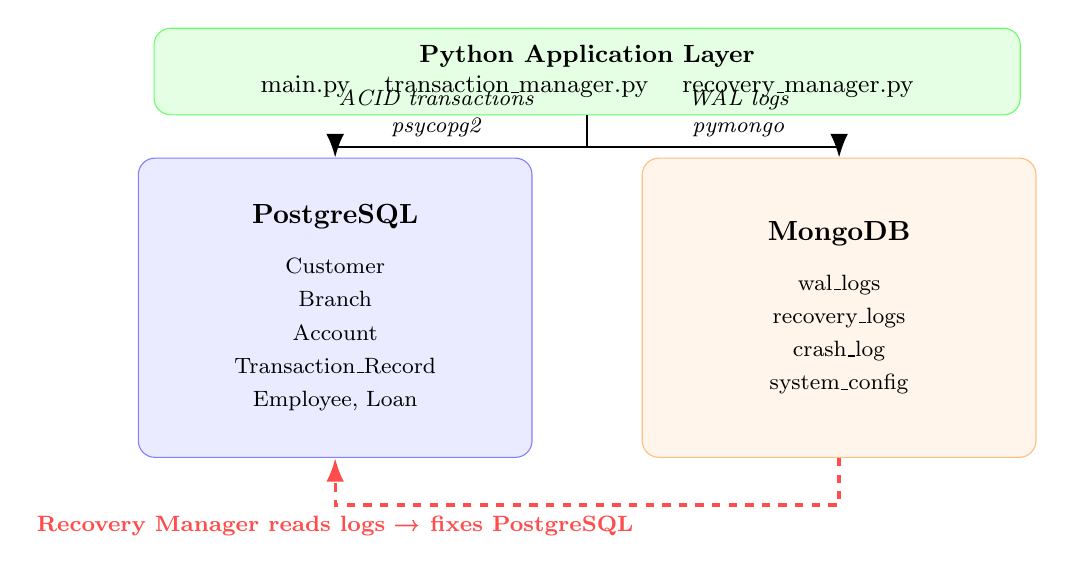
\begin{tikzpicture}[
  box/.style    = {draw, rounded corners=6pt, minimum width=5.5cm,
                   minimum height=1.1cm, align=center, font=\small},
  dbbox/.style  = {draw, rounded corners=6pt, minimum width=5cm,
                   minimum height=3.8cm, align=center},
  arr/.style    = {-{Latex[length=3mm]}, thick},
  label/.style  = {font=\footnotesize\itshape, align=center},
]

% Application layer
\node[box, fill=green!10, draw=green!60, minimum width=11cm]
  (app) at (0, 4.5) {\textbf{Python Application Layer}\\
  \small main.py \quad transaction\_manager.py \quad recovery\_manager.py};

% PostgreSQL box
\node[dbbox, fill=blue!8, draw=blue!50] (pg) at (-3.2, 1.5) {
  \textbf{PostgreSQL}\\[6pt]
  \footnotesize Customer\\
  \footnotesize Branch\\
  \footnotesize Account\\
  \footnotesize Transaction\_Record\\
  \footnotesize Employee, Loan
};

% MongoDB box
\node[dbbox, fill=orange!8, draw=orange!50] (mg) at (3.2, 1.5) {
  \textbf{MongoDB}\\[6pt]
  \footnotesize wal\_logs\\
  \footnotesize recovery\_logs\\
  \footnotesize crash\_log\\
  \footnotesize system\_config
};

% Arrows
\draw[arr] (app.south) -- ++(0,-0.4) -| (pg.north)
  node[pos=0.3, above, label] {ACID transactions\\psycopg2};
\draw[arr] (app.south) -- ++(0,-0.4) -| (mg.north)
  node[pos=0.3, above, label] {WAL logs\\pymongo};

% WAL arrow
\draw[arr, dashed, color=red!70, very thick]
  (mg.south) -- ++(0,-0.6) -| (pg.south)
  node[midway, below, font=\footnotesize\bfseries\color{red!70}]
  {Recovery Manager reads logs → fixes PostgreSQL};

\end{tikzpicture}
\caption{System Architecture: Python coordinates PostgreSQL and MongoDB}
\label{fig:architecture}
\end{figure}

\section{Component Roles}

\subsection{PostgreSQL --- Data Store}
PostgreSQL serves as the ground truth for banking data. It holds:
\begin{itemize}
  \item Current account balances (the data being protected)
  \item Transaction history records
  \item Customer, Branch, Employee, and Loan information
\end{itemize}
PostgreSQL transactions are controlled manually with explicit
\texttt{conn.commit()} and \texttt{conn.rollback()} calls.

\subsection{MongoDB --- WAL Log Store}
MongoDB stores Write-Ahead Log documents. Each document captures:
\begin{itemize}
  \item The \textit{old\_balance} before the change (used for UNDO)
  \item The \textit{new\_balance} after the change (used for REDO)
  \item The transaction status: \texttt{UNCOMMITTED}, \texttt{COMMITTED},
        or \texttt{ROLLED\_BACK}
\end{itemize}
MongoDB is used independently of the PostgreSQL transaction --- a failed
PG transaction does not affect the MongoDB log entry.

\subsection{Python Recovery Module}
Five Python modules coordinate the system:

\begin{table}[H]
\centering
\caption{Python Module Responsibilities}
\begin{tabularx}{\textwidth}{llX}
\toprule
\textbf{File} & \textbf{Class} & \textbf{Responsibility} \\
\midrule
db\_config.py & --- & PostgreSQL and MongoDB connection functions \\
mongo\_logger.py & MongoLogger & WAL log writes, updates, queries \\
transaction\_manager.py & TransactionManager & Deposit, withdraw, transfer with WAL \\
crash\_simulator.py & CrashSimulator & Mid-transaction crash injection \\
recovery\_manager.py & RecoveryManager & UNDO + REDO + Analysis phases \\
main.py & --- & Interactive menu-driven demo interface \\
\bottomrule
\end{tabularx}
\end{table}

\section{WAL Data Flow}

\begin{figure}[H]
\centering
\begin{tikzpicture}[
  step/.style = {draw, rounded corners=4pt, fill=gray!10,
                 minimum width=10cm, minimum height=0.8cm,
                 align=center, font=\small},
  crash/.style = {draw, rounded corners=4pt, fill=red!15, draw=red!60,
                  minimum width=10cm, minimum height=0.8cm,
                  align=center, font=\small\bfseries},
  arr/.style  = {-{Latex[length=3mm]}, thick},
]
\node[step]   (s1) at (0, 6)    {1. Read old\_balance from PostgreSQL};
\node[step, fill=yellow!20, draw=orange!70] (s2) at (0, 4.8)
  {\textbf{2. Write WAL log to MongoDB (status = UNCOMMITTED)} $\leftarrow$ WAL written FIRST};
\node[step]   (s3) at (0, 3.6)  {3. Update Account balance in PostgreSQL};
\node[step]   (s4) at (0, 2.4)  {4. Insert Transaction\_Record in PostgreSQL};
\node[step]   (s5) at (0, 1.2)  {5. conn.commit() --- PostgreSQL COMMIT};
\node[step, fill=green!15, draw=green!60]
              (s6) at (0, 0)    {6. Update MongoDB WAL log (status = COMMITTED)};
\node[crash]  (cx) at (6.5, 2.8) {$\Uparrow$ CRASH here\\leaves log UNCOMMITTED};

\draw[arr] (s1)--(s2); \draw[arr] (s2)--(s3);
\draw[arr] (s3)--(s4); \draw[arr] (s4)--(s5); \draw[arr] (s5)--(s6);
\draw[->, dashed, red!70, thick] (cx.west) -- (s3.east);
\end{tikzpicture}
\caption{WAL Transaction Sequence --- 6 steps}
\label{fig:wal_flow}
\end{figure}

% ────────────────────────────────────────────────────────────
\chapter{Entity-Relationship Diagram}

\section{ER Diagram Overview}

The database schema consists of six entities with the following relationships:

\begin{figure}[H]
\centering
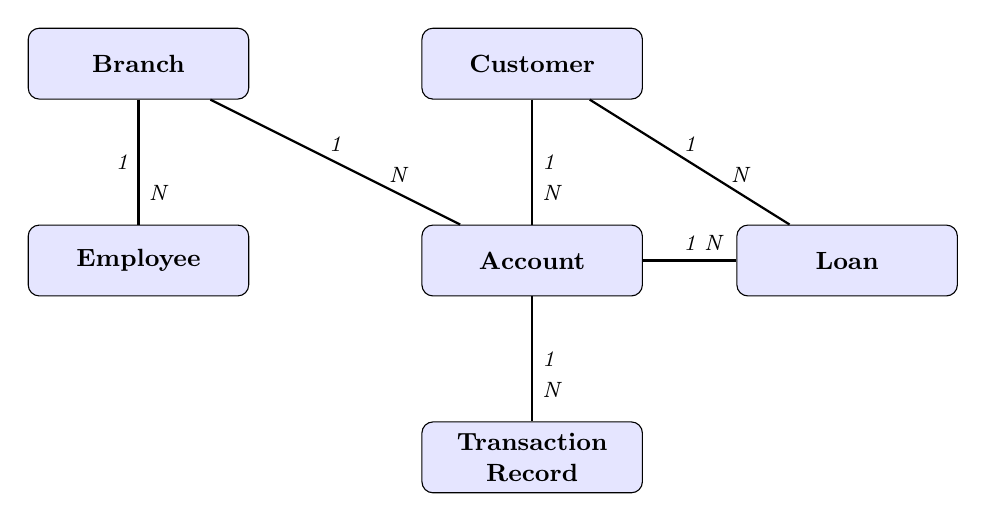
\begin{tikzpicture}[
  entity/.style = {draw, rectangle, rounded corners=4pt,
                   fill=blue!10, minimum width=2.8cm,
                   minimum height=0.9cm, align=center, font=\small\bfseries},
  rel/.style    = {font=\footnotesize\itshape},
  arr/.style    = {thick},
]
% Entities
\node[entity] (branch)   at (0, 6)    {Branch};
\node[entity] (customer) at (5, 6)    {Customer};
\node[entity] (employee) at (0, 3.5)  {Employee};
\node[entity] (account)  at (5, 3.5)  {Account};
\node[entity] (txn)      at (5, 1)    {Transaction\\Record};
\node[entity] (loan)     at (9, 3.5)  {Loan};

% Relationships
\draw[arr] (branch)   -- node[rel, left]  {1}  (employee)
           node[rel, right, near end] {N} {};
\draw[arr] (branch)   -- node[rel, above] {1}  (account)
           node[rel, above, near end] {N} {};
\draw[arr] (customer) -- node[rel, right] {1}  (account)
           node[rel, right, near end] {N} {};
\draw[arr] (account)  -- node[rel, right] {1}  (txn)
           node[rel, right, near end] {N} {};
\draw[arr] (customer) -- node[rel, above] {1}  (loan)
           node[rel, above, near end] {N} {};
\draw[arr] (account)  -- node[rel, above] {1}  (loan)
           node[rel, above, near end] {N} {};
\end{tikzpicture}
\caption{Entity-Relationship Diagram}
\label{fig:er}
\end{figure}

\section{Relationships and Cardinality}

\begin{table}[H]
\centering
\caption{Entity Relationships}
\begin{tabularx}{\textwidth}{llX}
\toprule
\textbf{Entity 1} & \textbf{Entity 2} & \textbf{Relationship} \\
\midrule
Branch   & Employee           & One branch employs many employees (1:N) \\
Branch   & Account            & One branch hosts many accounts (1:N) \\
Customer & Account            & One customer can have many accounts (1:N) \\
Account  & Transaction\_Record & One account has many transactions (1:N) \\
Customer & Loan               & One customer can have many loans (1:N) \\
Account  & Loan               & One account linked to many loans (1:N) \\
\bottomrule
\end{tabularx}
\end{table}

\section{Normalization}

The schema is normalized to \textbf{Third Normal Form (3NF)}:

\begin{itemize}
  \item \textbf{1NF}: All attributes are atomic. No multi-valued fields.
  \item \textbf{2NF}: No partial dependencies. All non-key attributes depend
        fully on the primary key.
  \item \textbf{3NF}: No transitive dependencies. Branch information is stored
        in the Branch table, not repeated in Account or Employee.
\end{itemize}

% ============================================================
% ch03_database_design.tex
% PostgreSQL Schema + MongoDB WAL Design
% ============================================================

\chapter{PostgreSQL Database Design}

\section{Schema Overview}

The PostgreSQL database \texttt{bank\_recovery\_db} contains six tables.
The \texttt{old\_balance} and \texttt{new\_balance} columns in
\texttt{Transaction\_Record} are critical --- they mirror the WAL log fields
and enable recovery directly from the relational database when needed.

\section{Table Definitions}

\subsection{Branch Table}

\begin{lstlisting}[style=sqlstyle, caption={Branch Table}]
CREATE TABLE Branch (
    branch_id      SERIAL       PRIMARY KEY,
    branch_name    VARCHAR(100) NOT NULL,
    branch_city    VARCHAR(50)  NOT NULL,
    branch_address TEXT,
    contact_number VARCHAR(20),
    created_at     TIMESTAMP    DEFAULT CURRENT_TIMESTAMP,
    CONSTRAINT chk_branch_name CHECK (TRIM(branch_name) <> '')
);
\end{lstlisting}

\subsection{Customer Table}

\begin{lstlisting}[style=sqlstyle, caption={Customer Table}]
CREATE TABLE Customer (
    customer_id    SERIAL       PRIMARY KEY,
    first_name     VARCHAR(50)  NOT NULL,
    last_name      VARCHAR(50)  NOT NULL,
    email          VARCHAR(100) UNIQUE NOT NULL,
    contact_number VARCHAR(20),
    address        TEXT,
    date_of_birth  DATE,
    created_at     TIMESTAMP    DEFAULT CURRENT_TIMESTAMP,
    CONSTRAINT chk_email CHECK (email LIKE '%@%.%'),
    CONSTRAINT chk_dob   CHECK (date_of_birth < CURRENT_DATE)
);
\end{lstlisting}

\subsection{Account Table}

\begin{lstlisting}[style=sqlstyle, caption={Account Table --- Core Banking Entity}]
CREATE TABLE Account (
    account_id     SERIAL        PRIMARY KEY,
    customer_id    INT           NOT NULL,
    branch_id      INT           NOT NULL,
    account_number VARCHAR(20)   UNIQUE NOT NULL,
    account_type   VARCHAR(30)   DEFAULT 'SAVINGS',
    balance        DECIMAL(12,2) DEFAULT 0.00,
    status         VARCHAR(20)   DEFAULT 'ACTIVE',
    created_at     TIMESTAMP     DEFAULT CURRENT_TIMESTAMP,
    CONSTRAINT fk_account_customer
        FOREIGN KEY (customer_id) REFERENCES Customer(customer_id)
        ON DELETE RESTRICT,
    CONSTRAINT fk_account_branch
        FOREIGN KEY (branch_id) REFERENCES Branch(branch_id)
        ON DELETE RESTRICT,
    CONSTRAINT chk_account_type
        CHECK (account_type IN ('SAVINGS','CURRENT','FIXED_DEPOSIT')),
    CONSTRAINT chk_account_status
        CHECK (status IN ('ACTIVE','INACTIVE','FROZEN','CLOSED')),
    CONSTRAINT chk_balance CHECK (balance >= 0.00)
);
\end{lstlisting}

\subsection{Transaction\_Record Table}

\begin{lstlisting}[style=sqlstyle, caption={Transaction\_Record --- WAL-mirroring balance columns}]
CREATE TABLE Transaction_Record (
    transaction_id     SERIAL        PRIMARY KEY,
    account_id         INT           NOT NULL,
    transaction_type   VARCHAR(20),
    amount             DECIMAL(12,2) NOT NULL CHECK (amount > 0),
    old_balance        DECIMAL(12,2) NOT NULL, -- Used in UNDO
    new_balance        DECIMAL(12,2) NOT NULL, -- Used in REDO
    transaction_status VARCHAR(20)   DEFAULT 'PENDING',
    transaction_time   TIMESTAMP     DEFAULT CURRENT_TIMESTAMP,
    notes              TEXT,
    CONSTRAINT fk_transaction_account
        FOREIGN KEY (account_id) REFERENCES Account(account_id),
    CONSTRAINT chk_txn_type
        CHECK (transaction_type IN
              ('DEPOSIT','WITHDRAWAL','TRANSFER_IN','TRANSFER_OUT')),
    CONSTRAINT chk_txn_status
        CHECK (transaction_status IN
              ('PENDING','COMMITTED','ROLLED_BACK'))
);
\end{lstlisting}

\begin{conceptbox}
\textbf{Key Design Decision:} \texttt{old\_balance} and \texttt{new\_balance}
are stored in \texttt{Transaction\_Record} and also in the MongoDB WAL log.
This redundancy is intentional --- it means recovery can use either source
to identify what to undo or redo.
\end{conceptbox}

\subsection{Employee Table}

\begin{lstlisting}[style=sqlstyle, caption={Employee Table}]
CREATE TABLE Employee (
    employee_id    SERIAL      PRIMARY KEY,
    branch_id      INT         NOT NULL,
    first_name     VARCHAR(50) NOT NULL,
    last_name      VARCHAR(50) NOT NULL,
    role           VARCHAR(50) DEFAULT 'TELLER',
    email          VARCHAR(100) UNIQUE,
    hire_date      DATE,
    CONSTRAINT fk_employee_branch
        FOREIGN KEY (branch_id) REFERENCES Branch(branch_id),
    CONSTRAINT chk_role
        CHECK (role IN ('MANAGER','TELLER','LOAN_OFFICER','CASHIER'))
);
\end{lstlisting}

\subsection{Loan Table}

\begin{lstlisting}[style=sqlstyle, caption={Loan Table}]
CREATE TABLE Loan (
    loan_id       SERIAL        PRIMARY KEY,
    customer_id   INT           NOT NULL,
    account_id    INT           NOT NULL,
    loan_type     VARCHAR(50)   DEFAULT 'PERSONAL',
    loan_amount   DECIMAL(12,2) NOT NULL CHECK (loan_amount > 0),
    interest_rate DECIMAL(5,2)  NOT NULL,
    start_date    DATE,
    end_date      DATE,
    loan_status   VARCHAR(20)   DEFAULT 'ACTIVE',
    CONSTRAINT fk_loan_customer
        FOREIGN KEY (customer_id) REFERENCES Customer(customer_id),
    CONSTRAINT fk_loan_account
        FOREIGN KEY (account_id) REFERENCES Account(account_id),
    CONSTRAINT chk_loan_type
        CHECK (loan_type IN ('HOME','CAR','PERSONAL','EDUCATION','BUSINESS')),
    CONSTRAINT chk_loan_status
        CHECK (loan_status IN ('ACTIVE','CLOSED','DEFAULTED'))
);
\end{lstlisting}

\section{Sample Data}

\begin{lstlisting}[style=sqlstyle, caption={Sample INSERT statements}]
-- Branch
INSERT INTO Branch (branch_name, branch_city, branch_address)
VALUES ('Main Branch', 'Lahore', '12 Mall Road, Lahore');

-- Customer
INSERT INTO Customer (first_name, last_name, email, date_of_birth)
VALUES ('Ali', 'Raza', 'ali.raza@gmail.com', '1990-03-15');

-- Account
INSERT INTO Account (customer_id, branch_id, account_number,
                     account_type, balance)
VALUES (1, 1, 'ACC-00001', 'SAVINGS', 10000.00);

-- Transaction with both balance fields (for recovery)
INSERT INTO Transaction_Record
    (account_id, transaction_type, amount,
     old_balance, new_balance, transaction_status, notes)
VALUES (1, 'DEPOSIT', 2000.00, 8000.00, 10000.00,
        'COMMITTED', 'Initial deposit');
\end{lstlisting}

% ────────────────────────────────────────────────────────────
\chapter{MongoDB WAL Design}

\section{Database and Collections}

MongoDB database: \texttt{bank\_recovery\_logs}

\begin{table}[H]
\centering
\caption{MongoDB Collections}
\begin{tabularx}{\textwidth}{llX}
\toprule
\textbf{Collection} & \textbf{Written By} & \textbf{Purpose} \\
\midrule
wal\_logs       & MongoLogger (every transaction) & WAL entries — one per operation \\
recovery\_logs  & RecoveryManager                 & Audit trail of UNDO/REDO actions \\
crash\_log      & CrashSimulator                  & Crash event records \\
system\_config  & MongoLogger                     & log\_id auto-increment counter \\
\bottomrule
\end{tabularx}
\end{table}

\section{wal\_logs Document Structure}

\begin{lstlisting}[style=jsonstyle, caption={WAL Log Document --- UNCOMMITTED state (after crash)}]
{
  "log_id":      8,
  "session_id":  "crash_a1b2c3",
  "account_id":  1,
  "txn_type":    "WITHDRAWAL",
  "old_balance": 10000.00,
  "new_balance":  7000.00,
  "amount":       3000.00,
  "status":      "UNCOMMITTED",
  "timestamp":   "2026-05-20T08:00:00Z",
  "notes":       "CRASH_DEMO: will not commit"
}
\end{lstlisting}

\begin{lstlisting}[style=jsonstyle, caption={WAL Log Document --- COMMITTED state (normal flow)}]
{
  "log_id":      1,
  "session_id":  "sess_f3a7b1",
  "account_id":  1,
  "txn_type":    "DEPOSIT",
  "old_balance": 8000.00,
  "new_balance": 10000.00,
  "amount":      2000.00,
  "status":      "COMMITTED",
  "timestamp":   "2026-05-20T08:00:00Z",
  "notes":       "Deposit to ACC-00001"
}
\end{lstlisting}

\section{Transaction Status Lifecycle}

\begin{figure}[H]
\centering
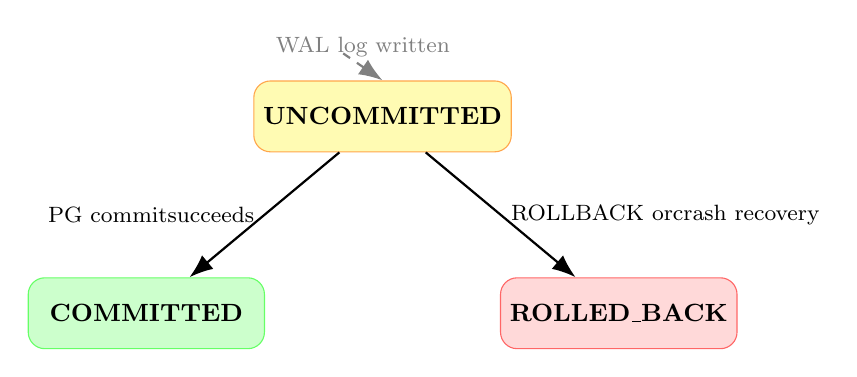
\begin{tikzpicture}[
  state/.style = {draw, rounded corners=6pt,
                  minimum width=3cm, minimum height=0.9cm,
                  align=center, font=\small\bfseries},
  arr/.style   = {-{Latex[length=3mm]}, thick},
]
\node[state, fill=yellow!30, draw=orange!70]
  (un) at (0,0)   {UNCOMMITTED};
\node[state, fill=green!20, draw=green!60]
  (co) at (-3,-2.5) {COMMITTED};
\node[state, fill=red!15,  draw=red!60]
  (rb) at (3, -2.5) {ROLLED\_BACK};

\draw[arr] (un) -- node[left, font=\footnotesize]
  {PG commit\\succeeds} (co);
\draw[arr] (un) -- node[right, font=\footnotesize]
  {ROLLBACK or\\crash recovery} (rb);
\draw[arr, dashed, gray] (-0.5, 0.8) -- node[above, font=\footnotesize]
  {WAL log written} (un.north);
\end{tikzpicture}
\caption{WAL Log Status Lifecycle}
\label{fig:status}
\end{figure}

\section{recovery\_logs Document}

\begin{lstlisting}[style=jsonstyle, caption={Recovery Log --- written by RecoveryManager after UNDO}]
{
  "action":      "UNDO",
  "account_id":  1,
  "before_bal":  7000.00,
  "after_bal":   10000.00,
  "reason":      "CRASH_DETECTED",
  "timestamp":   "2026-05-20T08:01:00Z"
}
\end{lstlisting}

\section{Useful MongoDB Queries}

\begin{lstlisting}[style=jsonstyle, caption={Key mongosh queries for demo and viva}]
// Find all UNCOMMITTED logs (crash victims)
db.wal_logs.find({ status: "UNCOMMITTED" })

// Find all COMMITTED logs
db.wal_logs.find({ status: "COMMITTED" })

// Count by status (shows system state at a glance)
db.wal_logs.aggregate([
    { $group: { _id: "$status", count: { $sum: 1 } } }
])

// Show UNDO plan: what to restore for each crash victim
db.wal_logs.find(
    { status: "UNCOMMITTED" },
    { log_id:1, account_id:1, old_balance:1, _id:0 }
)

// View all recovery actions taken
db.recovery_logs.find({}, { _id: 0 })
\end{lstlisting}

\section{Why MongoDB for WAL Logs?}

\begin{table}[H]
\centering
\caption{PostgreSQL vs MongoDB for Log Storage}
\begin{tabularx}{\textwidth}{lXX}
\toprule
\textbf{Criterion} & \textbf{PostgreSQL} & \textbf{MongoDB} \\
\midrule
Schema flexibility & Fixed columns only & Any fields per document \\
Insert speed & Transaction overhead & Lightweight insert \\
Log independence & Affected by PG crash & Independent of PG failures \\
Readability & Binary/SQL format & Human-readable JSON \\
Query language & SQL & Rich document queries \\
Status updates & UPDATE statement & \$set operator \\
\bottomrule
\end{tabularx}
\end{table}

% ============================================================
% ch04_implementation.tex
% WAL, Undo/Redo, Crash Simulation, Python Modules
% ============================================================

\chapter{Write-Ahead Logging Implementation}

\section{The WAL Protocol}

Every transaction in this system follows a strict 6-step sequence defined
in \texttt{transaction\_manager.py}. Steps must execute in this exact order:

\begin{table}[H]
\centering
\caption{WAL Transaction Steps}
\begin{tabularx}{\textwidth}{clX}
\toprule
\textbf{Step} & \textbf{Action} & \textbf{Details} \\
\midrule
1 & Read old\_balance & SELECT balance FROM Account WHERE account\_id = X \\
2 & \textbf{Write WAL log} & MongoDB insert (status=UNCOMMITTED) --- BEFORE any PG change \\
3 & Update PostgreSQL & UPDATE Account SET balance = new\_balance \\
4 & Insert Transaction\_Record & Records both old and new balance values \\
5 & conn.commit() & PostgreSQL transaction finalized \\
6 & mark\_committed() & MongoDB log updated to COMMITTED \\
\bottomrule
\end{tabularx}
\end{table}

\section{Deposit Implementation}

\begin{lstlisting}[style=pythonstyle, caption={Deposit method --- WAL sequence in Python}]
def deposit(self, account_number, amount, notes=""):
    conn   = get_pg_connection()
    cur    = conn.cursor()
    log_id = None
    try:
        # Step 1: Read old balance
        acc_id, old_bal = self._get_account(cur, account_number)
        new_bal = old_bal + amount

        # Step 2: Write WAL log BEFORE PostgreSQL update (WAL rule)
        log_id = self.logger.write_log(
            session_id  = self.session_id,
            account_id  = acc_id,
            txn_type    = "DEPOSIT",
            old_balance = old_bal,      # stored for UNDO
            new_balance = new_bal,      # stored for REDO
            amount      = amount,
        )

        # Step 3: Update PostgreSQL balance
        cur.execute("UPDATE Account SET balance = %s WHERE account_id = %s",
                    (new_bal, acc_id))

        # Step 4: Insert Transaction_Record
        self._record_transaction(cur, acc_id, "DEPOSIT",
                                 amount, old_bal, new_bal)

        # Step 5: COMMIT PostgreSQL
        conn.commit()

        # Step 6: Update WAL log to COMMITTED
        self.logger.mark_committed(log_id)

    except Exception as e:
        conn.rollback()                        # Reverse all PG changes
        if log_id:
            self.logger.mark_rolled_back(log_id, reason=str(e))
    finally:
        cur.close(); conn.close()
\end{lstlisting}

\section{Transfer --- Atomic Two-Leg Transaction}

A fund transfer involves two accounts and demonstrates ACID Atomicity:
both legs commit together or both are rolled back together.

\begin{lstlisting}[style=pythonstyle, caption={Transfer --- two WAL logs, one PG commit}]
# Step 2: Write BOTH WAL logs BEFORE any PostgreSQL update
log_out_id = self.logger.write_log(
    account_id=from_id, txn_type="TRANSFER_OUT",
    old_balance=from_bal, new_balance=from_new, amount=amount
)
log_in_id = self.logger.write_log(
    account_id=to_id, txn_type="TRANSFER_IN",
    old_balance=to_bal, new_balance=to_new, amount=amount
)

# Step 3: Apply both PostgreSQL updates
cur.execute("UPDATE Account SET balance=%s WHERE account_id=%s",
            (from_new, from_id))
cur.execute("UPDATE Account SET balance=%s WHERE account_id=%s",
            (to_new, to_id))

# Step 5: ONE commit covers both updates (Atomicity)
conn.commit()

# Step 6: Mark both WAL logs COMMITTED
self.logger.mark_committed(log_out_id)
self.logger.mark_committed(log_in_id)
\end{lstlisting}

% ────────────────────────────────────────────────────────────
\chapter{Crash Simulation}

\section{How a Crash is Simulated}

In \texttt{crash\_simulator.py}, a \texttt{RuntimeError} is raised between
Step 3 (PG update) and Step 5 (PG commit). This creates the same state
that a real OS crash would leave:

\begin{lstlisting}[style=pythonstyle, caption={crash\_simulator.py --- crash injection point}]
def simulate_crash(self, account_number, amount, txn_type="WITHDRAWAL"):
    conn   = get_pg_connection()
    cur    = conn.cursor()
    log_id = None
    try:
        acc_id, old_bal = _get_account(cur, account_number)
        new_bal = old_bal - amount

        # Step 2: WAL log written (UNCOMMITTED) --- this PERSISTS
        log_id = self.logger.write_log(
            session_id=self.session_id, account_id=acc_id,
            txn_type=txn_type, old_balance=old_bal,
            new_balance=new_bal, amount=amount,
            notes="CRASH_DEMO: will not commit"
        )

        # Step 3: PG balance changed
        cur.execute("UPDATE Account SET balance=%s WHERE account_id=%s",
                    (new_bal, acc_id))

        # *** CRASH HERE --- before conn.commit() ***
        raise RuntimeError("SIMULATED CRASH")

    except RuntimeError:
        conn.rollback()     # PG auto-rolls back (connection drop)
        # MongoDB log stays UNCOMMITTED <- recovery target
        return log_id
\end{lstlisting}

\section{State After Crash}

After \texttt{simulate\_crash()} returns:

\begin{table}[H]
\centering
\caption{Database State After Crash}
\begin{tabularx}{\textwidth}{lX}
\toprule
\textbf{Database} & \textbf{State} \\
\midrule
MongoDB wal\_logs & Log entry exists with \texttt{status = "UNCOMMITTED"} \\
PostgreSQL Account & Balance is restored to old\_balance (PG auto-rollback) \\
PostgreSQL Transaction\_Record & No record exists (INSERT was in the same transaction) \\
\bottomrule
\end{tabularx}
\end{table}

\begin{conceptbox}
\textbf{Important distinction for viva:}
In our simulation, PostgreSQL auto-rolls-back because we close the connection.
In a real crash, the OS terminates the process and PostgreSQL detects the
lost connection during its next startup. The MongoDB log remains UNCOMMITTED
in both cases --- that is the key state the Recovery Manager reads.
\end{conceptbox}

% ────────────────────────────────────────────────────────────
\chapter{Recovery Manager}

\section{Three-Phase Recovery}

The \texttt{RecoveryManager} implements a simplified ARIES-inspired process
in three sequential phases:

\begin{lstlisting}[style=pythonstyle, caption={recovery\_manager.py --- main entry point}]
def run_recovery(self):
    # Phase 1: Analysis
    uncommitted, committed = self._phase_analysis()

    # Phase 2: UNDO uncommitted transactions
    undo_count = self._phase_undo(uncommitted)

    # Phase 3: REDO committed transactions if PG state is wrong
    redo_count = self._phase_redo(committed)
\end{lstlisting}

\section{Phase 1: Analysis}

Reads all WAL logs from MongoDB and classifies them:

\begin{lstlisting}[style=pythonstyle, caption={Analysis phase}]
def _phase_analysis(self):
    uncommitted = self.logger.get_uncommitted()  # status="UNCOMMITTED"
    committed   = self.logger.get_committed()    # status="COMMITTED"
    return uncommitted, committed
\end{lstlisting}

\section{Phase 2: UNDO}

For each UNCOMMITTED log (newest first), restores \texttt{old\_balance}:

\begin{lstlisting}[style=pythonstyle, caption={UNDO phase --- restore old\_balance}]
def _phase_undo(self, uncommitted_logs):
    for log in uncommitted_logs:
        acc_id      = log["account_id"]
        old_balance = log["old_balance"]   # <- from WAL log
        log_id      = log["log_id"]

        # Read current PG balance
        cur.execute("SELECT balance FROM Account WHERE account_id=%s",
                    (acc_id,))
        pg_balance = float(cur.fetchone()[0])

        # Idempotency: skip if already restored
        if abs(pg_balance - old_balance) < 0.001:
            self.logger.mark_rolled_back(log_id, "Already restored")
            continue

        # Apply UNDO: restore old_balance in PostgreSQL
        cur.execute("UPDATE Account SET balance=%s WHERE account_id=%s",
                    (old_balance, acc_id))
        conn.commit()

        # Update WAL log -> ROLLED_BACK
        self.logger.mark_rolled_back(log_id, "UNDO by RecoveryManager")

        # Write recovery audit entry
        self.logger.write_recovery_log(
            action="UNDO", account_id=acc_id,
            before_bal=pg_balance, after_bal=old_balance,
            reason="CRASH_DETECTED"
        )
\end{lstlisting}

\section{Phase 3: REDO}

For each COMMITTED log, checks if PostgreSQL already reflects the committed
change. If not, re-applies \texttt{new\_balance}:

\begin{lstlisting}[style=pythonstyle, caption={REDO phase --- re-apply new\_balance if PG state is wrong}]
def _phase_redo(self, committed_logs):
    for log in committed_logs:
        acc_id      = log["account_id"]
        new_balance = log["new_balance"]   # <- from WAL log

        cur.execute("SELECT balance FROM Account WHERE account_id=%s",
                    (acc_id,))
        pg_balance = float(cur.fetchone()[0])

        # If PG already matches -> no REDO needed (idempotent)
        if abs(pg_balance - new_balance) < 0.001:
            continue

        # REDO: re-apply new_balance
        cur.execute("UPDATE Account SET balance=%s WHERE account_id=%s",
                    (new_balance, acc_id))
        conn.commit()

        self.logger.write_recovery_log(
            action="REDO", account_id=acc_id,
            before_bal=pg_balance, after_bal=new_balance,
            reason="COMMIT_LOSS"
        )
\end{lstlisting}

\section{Idempotency}

A key property of the recovery process is \textbf{idempotency} --- running
recovery multiple times produces the same result as running it once.

\begin{itemize}
  \item \textbf{UNDO idempotency}: If PG balance already equals
        \texttt{old\_balance}, UNDO is skipped.
  \item \textbf{REDO idempotency}: If PG balance already equals
        \texttt{new\_balance}, REDO is skipped.
\end{itemize}

This ensures the Recovery Manager is safe to run even if it is interrupted
partway through.

% ────────────────────────────────────────────────────────────
\chapter{Python Module Explanation}

\section{Module Overview}

\begin{table}[H]
\centering
\caption{Python Modules and ADBMS Concepts}
\begin{tabularx}{\textwidth}{llX}
\toprule
\textbf{Module} & \textbf{Concept} & \textbf{Why it exists} \\
\midrule
db\_config.py & Polyglot Persistence & Central DB connection management \\
mongo\_logger.py & WAL & All MongoDB log operations in one place \\
transaction\_manager.py & Transactions, ACID & Enforces WAL sequence for every transaction \\
crash\_simulator.py & Crash Recovery & Creates testable inconsistency scenarios \\
recovery\_manager.py & UNDO/REDO, ARIES & Detects and repairs post-crash inconsistency \\
main.py & --- & Interactive demo runner for viva/presentation \\
\bottomrule
\end{tabularx}
\end{table}

\section{db\_config.py}

\begin{lstlisting}[style=pythonstyle, caption={db\_config.py --- connection functions}]
def get_pg_connection():
    conn = psycopg2.connect(host="localhost", dbname="bank_recovery_db",
                            user="postgres", password="your_password")
    conn.autocommit = False   # Manual transaction control
    return conn

def get_mongo_db():
    client = MongoClient("mongodb://localhost:27017/")
    return client["bank_recovery_logs"]
\end{lstlisting}

\textbf{ADBMS Concept:} \texttt{autocommit=False} is the key setting.
It means every SQL statement is inside an implicit transaction until we
call \texttt{conn.commit()} or \texttt{conn.rollback()}.

\section{mongo\_logger.py}

The \texttt{write\_log()} method is the heart of the WAL system:

\begin{lstlisting}[style=pythonstyle, caption={MongoLogger.write\_log() --- WAL insert}]
def write_log(self, session_id, account_id, txn_type,
              old_balance, new_balance, amount, notes=""):
    log_id = self._next_log_id()
    self.col.insert_one({
        "log_id":      log_id,
        "session_id":  session_id,
        "account_id":  account_id,
        "txn_type":    txn_type,
        "old_balance": float(old_balance),   # UNDO uses this
        "new_balance": float(new_balance),   # REDO uses this
        "amount":      float(amount),
        "status":      "UNCOMMITTED",        # Always starts UNCOMMITTED
        "timestamp":   datetime.now(timezone.utc),
        "notes":       notes,
    })
    return log_id
\end{lstlisting}

\section{main.py --- Demo Menu}

\begin{lstlisting}[style=pythonstyle, caption={main.py menu structure}]
actions = {
    "1": menu_deposit,     # WAL + COMMIT demo
    "2": menu_withdraw,    # WAL + COMMIT or ROLLBACK
    "3": menu_transfer,    # Two-leg atomic transfer
    "4": menu_crash,       # Crash before COMMIT
    "5": menu_recovery,    # UNDO + REDO phases
    "6": menu_show_logs,   # View MongoDB WAL logs
    "7": menu_show_balances, # View PostgreSQL balances
}
\end{lstlisting}

% ============================================================
% ch05_results.tex
% Demo Flow, Advantages, Limitations, Viva Preparation
% ============================================================

\chapter{Demonstration Flow}

\section{Recommended Viva Demo Sequence}

The following sequence demonstrates all ADBMS concepts within 10--15 minutes:

\begin{table}[H]
\centering
\caption{Demo Sequence for Viva}
\begin{tabularx}{\textwidth}{clX}
\toprule
\textbf{Step} & \textbf{Menu Option} & \textbf{Concept Shown} \\
\midrule
1 & 7 (Show Balances) & Starting PostgreSQL state \\
2 & 6 (Show WAL Logs) & Empty or existing MongoDB logs \\
3 & 1 (Deposit) & WAL written → PG updated → COMMITTED \\
4 & 6 (Show WAL Logs) & See the COMMITTED entry \\
5 & 2 (Withdraw, large amount) & Insufficient funds → ROLLBACK → ROLLED\_BACK \\
6 & 4 (Simulate Crash) & UNCOMMITTED log created in MongoDB \\
7 & 6 (Show WAL Logs) & Point to the UNCOMMITTED entry \\
8 & 7 (Show Balances) & Verify PG balance unchanged (auto-rollback) \\
9 & 5 (Run Recovery) & Analysis → UNDO → REDO phases \\
10 & 6 (Show WAL Logs) & Entry now ROLLED\_BACK \\
11 & 7 (Show Balances) & Consistent state confirmed \\
\bottomrule
\end{tabularx}
\end{table}

\section{Sample Terminal Output}

\subsection{Normal Deposit (Option 1)}

\begin{lstlisting}[style=jsonstyle, caption={Deposit terminal output}]
  [Session] sess_a1b2c3

  ====================================================
  DEPOSIT | ACC-00001 | +1500.00
  ====================================================
  Old balance: 10000.00
    [WAL] Log #1 -> UNCOMMITTED  (DEPOSIT, account=1, 10000.00->11500.00)
    [PG]  COMMIT -- Transaction_Record id=13
    [WAL] Log #1 -> COMMITTED
  New balance: 11500.00
  v Deposit successful.
\end{lstlisting}

\subsection{Rollback --- Insufficient Funds (Option 2)}

\begin{lstlisting}[style=jsonstyle, caption={Rollback terminal output}]
  ====================================================
  WITHDRAWAL | ACC-00005 | -50000.00
  ====================================================
  Old balance: 8000.00
    [WAL] Log #2 -> UNCOMMITTED  (WITHDRAWAL, account=5, 8000.00->-42000.00)
  [ERROR] Insufficient funds. Balance: 8000.00, Requested: 50000.00
  [PG] ROLLBACK -- balance unchanged.
    [WAL] Log #2 -> ROLLED_BACK
\end{lstlisting}

\subsection{Crash Simulation (Option 4)}

\begin{lstlisting}[style=jsonstyle, caption={Crash simulation terminal output}]
  ====================================================
  CRASH SIMULATION -- WITHDRAWAL
  Account : ACC-00001  |  Amount: 3000.00
  ====================================================
  Current balance: 11500.00
    [WAL] Log #3 -> UNCOMMITTED  (WITHDRAWAL, account=1, ...)
  [PG]  Balance changed: 11500.00 -> 8500.00
  [PG]  (Change applied but NOT yet committed)

  *** SYSTEM CRASH -- Exception raised! ***
  *** COMMIT was never executed.        ***

  [PG]  Connection closed -> PG auto-rollback
        (PG balance restored to 11500.00)
  [WAL] Log #3 still UNCOMMITTED in MongoDB
  -> Run Recovery Manager (option 5) to fix the database.
\end{lstlisting}

\subsection{Recovery Manager (Option 5)}

\begin{lstlisting}[style=jsonstyle, caption={Recovery Manager terminal output}]
  ####################################################
  RECOVERY MANAGER -- Starting Recovery
  ####################################################

  -- Phase 1: ANALYSIS --
  Scanning MongoDB WAL logs...
  Found 1 UNCOMMITTED log(s) -> need UNDO
  Found 5 COMMITTED   log(s) -> check REDO

  Crash victims (will be UNDONE):
    log_id=3  account_id=1  type=WITHDRAWAL  old=11500.00  new=8500.00

  -- Phase 2: UNDO --
  Restoring 1 account(s) to pre-crash state...

  UNDO log_id=3  account_id=1
    PG balance now : 11500.00
    Restoring to   : 11500.00  <- from WAL log
    Already at old_balance. UNDO already done. Skipping.

  -- Phase 3: REDO --
  v All committed transactions consistent. No REDO needed.

  ####################################################
  RECOVERY COMPLETE
  UNDO applied : 0   (PG already consistent -- auto-rollback handled it)
  REDO applied : 0
  PostgreSQL is now in a consistent state.
  ####################################################
\end{lstlisting}

% ────────────────────────────────────────────────────────────
\chapter{Advantages and Limitations}

\section{Advantages}

\begin{enumerate}
  \item \textbf{Educational Clarity}: Every step of WAL and recovery is
        visible in the terminal output. Students can trace exactly what
        happens to both databases at each transaction stage.

  \item \textbf{Polyglot Persistence}: Demonstrates a hybrid architecture
        where two databases complement each other --- a real-world pattern
        used in modern applications.

  \item \textbf{Practical Implementation}: The entire system runs on a
        single laptop using freely available software (PostgreSQL, MongoDB,
        Python).

  \item \textbf{Observable Recovery}: Unlike built-in DBMS recovery which
        is invisible to users, this system makes recovery explicit and
        observable through MongoDB queries and terminal output.

  \item \textbf{Idempotent Recovery}: The recovery manager can be run
        multiple times safely, demonstrating a key property of robust
        recovery systems.

  \item \textbf{Modular Design}: Each Python module is focused on one
        responsibility, making the code easy to understand, extend, and
        explain during viva.
\end{enumerate}

\section{Limitations}

\begin{enumerate}
  \item \textbf{Single-User Only}: The system does not handle concurrent
        transactions. Running two transactions simultaneously could
        produce incorrect results.

  \item \textbf{No Checkpoint Support}: A full ARIES implementation uses
        checkpoints to limit how far back in the log recovery must scan.
        Our system always scans all logs.

  \item \textbf{No LSN Chain}: Log Sequence Numbers link log records for
        ordered undo/redo. Our system uses timestamps and log\_id ordering,
        which is less precise.

  \item \textbf{Simplified Crash Model}: Our crash simulation uses a
        Python exception. A real crash (power loss, OS kill) has more
        complex storage-level effects.

  \item \textbf{No Page-Level Recovery}: Our system operates at the
        account/row level. Real DBMS recovery operates at the page level
        for finer-grained control.

  \item \textbf{MongoDB Not Crash-Safe by Default}: If MongoDB itself
        crashes before the log insert completes, the log is also lost.
        A production system would require MongoDB with journaling enabled
        and write concern set to ``majority''.
\end{enumerate}

% ────────────────────────────────────────────────────────────
\chapter{Viva Preparation}

\section{Expected Teacher Questions and Answers}

\subsection{Q1: What is Write-Ahead Logging?}

\textbf{Answer:} Write-Ahead Logging is the rule that a log record must be
written to stable storage \textit{before} the data change it describes is
applied. In our system, we insert a document into MongoDB's \texttt{wal\_logs}
collection before running the \texttt{UPDATE Account SET balance = ...}
statement in PostgreSQL. This guarantees that even if PostgreSQL crashes
mid-update, the log exists and we know what to undo.

\subsection{Q2: What is the difference between UNDO and REDO?}

\textbf{Answer:}
\begin{itemize}
  \item \textbf{UNDO}: Reverses an \textit{uncommitted} transaction by
        restoring \texttt{old\_balance} (read from the WAL log). Used for
        crash victims that never reached COMMIT.
  \item \textbf{REDO}: Re-applies a \textit{committed} transaction by
        applying \texttt{new\_balance} (from the WAL log). Used when a
        committed change was lost before being flushed to PostgreSQL disk.
\end{itemize}

\subsection{Q3: How do you identify uncommitted transactions after a crash?}

\textbf{Answer:} We query MongoDB for all documents where
\texttt{status = "UNCOMMITTED"}. These are transactions that wrote a WAL
log but never had their status updated to \texttt{COMMITTED} or
\texttt{ROLLED\_BACK} --- the crash happened between those steps.

\subsection{Q4: Why use MongoDB for WAL logs instead of PostgreSQL?}

\textbf{Answer:} MongoDB is used because:
(1) Log inserts are fast and lightweight without transaction overhead.
(2) MongoDB is independent of the PostgreSQL transaction --- a PG rollback
does not affect the MongoDB log.
(3) JSON documents are flexible and human-readable, making logs easy to
inspect and demonstrate.
(4) It demonstrates polyglot persistence --- using each database for what
it does best.

\subsection{Q5: What is ACID? How does your system demonstrate it?}

\textbf{Answer:}
\begin{itemize}
  \item \textbf{Atomicity}: Transfer uses one \texttt{conn.commit()} for
        both account updates. If one fails, both rollback.
  \item \textbf{Consistency}: CHECK constraints and FK constraints in
        PostgreSQL prevent invalid data (e.g., negative balance).
  \item \textbf{Isolation}: PostgreSQL handles concurrent isolation via
        its transaction model (one connection at a time in our demo).
  \item \textbf{Durability}: WAL log is written first, ensuring the
        operation can be recovered even after a crash.
\end{itemize}

\subsection{Q6: How is your recovery similar to ARIES?}

\textbf{Answer:} ARIES has three phases: Analysis, Redo, Undo. Our system
follows the same three phases. The difference is that ARIES uses Log Sequence
Numbers for precise ordering, maintains a dirty page table, and operates at
the page level. Our system uses timestamps and log\_id for ordering, operates
at the account row level, and is simplified for undergraduate demonstration.

\subsection{Q7: What is polyglot persistence?}

\textbf{Answer:} Polyglot persistence means using multiple database
technologies in one application, each chosen for its strengths. In our
system, PostgreSQL handles ACID-compliant relational banking data while
MongoDB handles flexible, fast-insert WAL log documents. Together they form
a more capable system than either alone.

\subsection{Q8: Show me the WAL log in MongoDB right after a crash.}

\textbf{Answer:} Run option 4 from the menu, then in mongosh run:
\begin{lstlisting}[style=jsonstyle]
use("bank_recovery_logs")
db.wal_logs.find({ status: "UNCOMMITTED" })
\end{lstlisting}
This shows the log entry written before the crash, still showing
\texttt{UNCOMMITTED} because the system never reached the COMMIT step.

\section{Key Concepts Quick Reference}

\begin{table}[H]
\centering
\caption{Quick Reference for Viva}
\begin{tabularx}{\textwidth}{lX}
\toprule
\textbf{Concept} & \textbf{One-line explanation} \\
\midrule
WAL & Log first, then update the database \\
UNCOMMITTED & Transaction started but crash happened before COMMIT \\
UNDO & Restore old\_balance to reverse an uncommitted transaction \\
REDO & Re-apply new\_balance for a committed but lost transaction \\
Atomicity & All steps of a transaction succeed or all are reversed \\
Durability & Committed data survives crashes (WAL makes this possible) \\
Polyglot & Two databases used together, each for its strength \\
Idempotency & Recovery gives same result whether run once or many times \\
\bottomrule
\end{tabularx}
\end{table}

% ============================================================
% ch06_conclusion.tex
% Conclusion, Future Enhancements, References
% ============================================================

\chapter{Conclusion}

This project successfully implemented a simplified \textbf{Log-Based Recovery
System} demonstrating core Advanced Database Management Systems concepts in a
practical, observable manner. The following objectives were achieved:

\begin{enumerate}
  \item \textbf{Write-Ahead Logging} was implemented using MongoDB as the
        WAL store. Every transaction writes a log entry before modifying
        PostgreSQL, ensuring that no data change is unlogged.

  \item \textbf{Transaction Management} was demonstrated through explicit
        deposit, withdrawal, and transfer operations with manual
        \texttt{COMMIT} and \texttt{ROLLBACK} control.

  \item \textbf{Crash Simulation} provided a testable way to create
        database inconsistency by injecting a failure between the WAL log
        write and the PostgreSQL commit.

  \item \textbf{UNDO Recovery} successfully identified UNCOMMITTED WAL
        logs and restored old balances in PostgreSQL, confirming the
        system's ability to reverse incomplete transactions.

  \item \textbf{REDO Recovery} verified that committed transactions whose
        PostgreSQL effects were lost could be re-applied from the WAL log.

  \item \textbf{Polyglot Persistence} was demonstrated by the coordinated
        use of PostgreSQL (relational, ACID) and MongoDB (document, flexible)
        in a single application.
\end{enumerate}

The project shows that recovery concepts traditionally explained through
complex theory can be made concrete and observable through a practical
implementation. The system is suitable for viva presentation and provides
a strong foundation for understanding how production databases handle
crash recovery.

\section{Future Enhancements}

The following enhancements would make the system more complete:

\begin{enumerate}
  \item \textbf{Checkpoint Support}: Implement periodic checkpoints to
        limit recovery scan range and improve performance for large log sets.

  \item \textbf{Log Sequence Numbers (LSN)}: Add LSN ordering to WAL logs
        for more precise undo/redo sequencing, moving closer to full ARIES.

  \item \textbf{Concurrent Transactions}: Add locking mechanisms to support
        multiple simultaneous users while maintaining data consistency.

  \item \textbf{Web Dashboard}: Build a simple Flask or FastAPI web interface
        to visualize WAL logs and recovery actions in a browser.

  \item \textbf{Compression and Archiving}: Implement log rotation and
        archiving for the MongoDB WAL collection to manage long-term storage.

  \item \textbf{Transfer Recovery}: Extend recovery to handle partial
        two-leg transfers where only one leg was applied before a crash.

  \item \textbf{MongoDB Write Concern}: Enable \texttt{w: "majority"} write
        concern to ensure WAL logs survive MongoDB node failures.
\end{enumerate}

% ────────────────────────────────────────────────────────────
\begin{thebibliography}{9}

\bibitem{ramakrishnan2002}
  Ramakrishnan, R. and Gehrke, J. (2002).
  \textit{Database Management Systems}, 3rd Edition.
  McGraw-Hill Education.

\bibitem{mohan1992}
  Mohan, C., Haderle, D., Lindsay, B., Pirahesh, H., and Schwarz, P. (1992).
  ARIES: A Transaction Recovery Method Supporting Fine-Granularity Locking
  and Partial Rollbacks Using Write-Ahead Logging.
  \textit{ACM Transactions on Database Systems}, 17(1), 94--162.

\bibitem{gray1993}
  Gray, J. and Reuter, A. (1993).
  \textit{Transaction Processing: Concepts and Techniques}.
  Morgan Kaufmann Publishers.

\bibitem{fowler2012}
  Fowler, M. and Sadalage, P.J. (2012).
  \textit{NoSQL Distilled: A Brief Guide to the Emerging World of
  Polyglot Persistence}.
  Addison-Wesley Professional.

\bibitem{postgresql2024}
  PostgreSQL Global Development Group. (2024).
  \textit{PostgreSQL 16 Documentation}.
  \url{https://www.postgresql.org/docs/16/}

\bibitem{mongodb2024}
  MongoDB, Inc. (2024).
  \textit{MongoDB Manual}.
  \url{https://www.mongodb.com/docs/manual/}

\bibitem{silberschatz2020}
  Silberschatz, A., Korth, H.F., and Sudarshan, S. (2020).
  \textit{Database System Concepts}, 7th Edition.
  McGraw-Hill Education.

\bibitem{psycopg2}
  Di Gregorio, F. (2024).
  \textit{Psycopg 2.9 Documentation}.
  \url{https://www.psycopg.org/docs/}

\bibitem{pymongo}
  MongoDB, Inc. (2024).
  \textit{PyMongo 4.6 Documentation}.
  \url{https://pymongo.readthedocs.io/}

\end{thebibliography}


\end{document}
